\documentclass{beamer}
\usetheme{VATT}
\usepackage[utf8]{inputenc}

\usepackage{todonotes}
\presetkeys{todonotes}{inline}{}


\title{team meeting}
\author{jjycavailles }
\date{June 2019}

\usepackage{natbib}
\usepackage{graphicx}


%\begin{center}
%  
\includegraphics[width = 25mm]{LogoInsa.png} \hfill
%  
\includegraphics[width = 30mm]{logo_cnrs.jpg}
%\end{center}

%\titlegraphic{
\includegraphics[width=2cm]{cnrs.png}}
%\title{
\includegraphics[width=2cm]{cnrs.png} \\ Destabilizing effects of controlling ecosystem behavior}
\title{Destabilizing effects \\ of controlling ecosystem behavior}
\subtitle{\it{ \rule{\linewidth}{0.5mm} \\ [0.4cm] \\ Jérôme Cavaillès}}
%\title{Destabilizing effects of controlling ecosystem behavior \\ \\ 
\includegraphics[width=4cm]{paul_sab.jpg} 
\includegraphics[width=1.5cm]{cnrs.png}}

%\title{Destabilizing effects \\ of controlling ecosystem behavior \\ 
%\begin{columns}
%\texorpdfstring{
       % \column{.33\linewidth}
      %  \centering
     %   
\includegraphics[width=4cm]{paul_sab.jpg}
    %    \column{.33\linewidth}
   %     \centering
  %      
\includegraphics[width=1.5cm]{cnrs.png}
 %   \end{columns}
%}       } 

%\subtitle{Projet 4GMM}
%\author{VATT Communication}
\author[Jérôme Cavaillès, Yuval Zelnik]{%
  \texorpdfstring{%
    \begin{columns}
      \column{.33\linewidth}
      \centering
      Supervisor \\ \it{Yuval Zelnik} \\ \it{Michel Loreau}
      \column{.33\linewidth}
      \centering
    University \\ INSA Toulouse \\ Paul Sabatier     
     % \column{.33\linewidth}
     % \centering
     % Author 3 \\ Institute 3
    \end{columns}
 }
 {Author 1, Author 2, Author 3}
}

%\date{\today}
\institute{%
  \texorpdfstring{%
    \begin{columns}
      \column{.9\linewidth}
      \centering
   %   \url{lcaselle@etud.insa-toulouse.fr} \\
    %  \url{jcavaill@etud.insa-toulouse.fr} \\
      %\url{firstname.lastname@institute3.com}
    \end{columns}
 }
 {Author 1, Author 2, Author 3}
}



\begin{document}


\begin{frame}[plain,t]
\titlepage
% add logo sur la page de présentation
\end{frame}



%\begin{frame}
%\frametitle{Contents} 
%\todo{content before of after context ?}
%\tableofcontents
%\end{frame}



\section{Context}

\subsection{ecosystem management}
\begin{frame}
\frametitle{Context} % PRESENT IN 2 COLUMNS ?
\begin{enumerate}
\item Overall goal : protect ecosystem
%\begin{itemize}
%    \item protect services of a forest (ex : wood production)
%\end{itemize}
\item[]
%$\Rightarrow$ 
\item Stabilize ecosystem 
%\begin{itemize}
%    \item wildfire reduction
%\end{itemize}
\item[]
\item Long term consequences 
%\begin{itemize}
%    \item dead wood accumulation
%\end{itemize}
\item[]
\item In some cases : collapse of the system 
%\begin{itemize}
%    \item more damaging fire
%\end{itemize}
\end{enumerate}
\end{frame}



\subsection{Forest fire management}
\begin{frame}
\frametitle{Forest fire management}
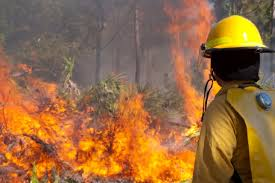
\includegraphics[width=8.cm]{forest_fire__fireman.jpg}
\end{frame}



\section{Methods}


\subsection{Model}



\begin{frame}
%\frametitle{Model of the forest \only<1>{growth}\only<2>{fire}}
\only<1>{\frametitle{Model of the forest growth}}
\only<2>{\frametitle{Model of the forest fire}}
\only<3>{\frametitle{Non-dimensionalisation Model}} % cancel{} ??
\[
\left\{
\begin{array}{rcl}
\frac{dN}{dt} & = & \onslide<1,2>{g}N(1-N\onslide<1,2>{/K})(N\onslide<1,2>{/A}-\only<1,2>{1}\only<3>{a}) \onslide<2->{+ \delta_F(t)s(t)(N+\alpha W)}\\
\\
\frac{dW}{dt} & = & \only<1,2>{\mu}\only<3>{m}N-dW  \onslide<2->{+ \beta\cdot\delta_F(t)s(t)\beta(N+\alpha W)}\\
\end{array}
\right.
\]
\only<1>{
\begin{itemize}
    \item N : living biomass
    \item W : death biomass
\end{itemize}
}
\only<2>{
\begin{itemize}
    \item F : frequency of the fire
    \item s : strength of the fire
\end{itemize}
}
\only<3>{
\begin{itemize}
    \item We adimensionalised the system
    \item 7 parameters remains
\end{itemize}
}
\end{frame}


% PRESENT "TIMES SERIES" HERE OTHERWISE MEASURES IS MORE DIFFICULT TO UNDERSTAND

\subsection{Measures}

\begin{frame}

\only<1>{
\frametitle{Time series}}
\only<2>{
\frametitle{Variability}}
\only<3>{
\frametitle{Collapse}}

\only<1>{
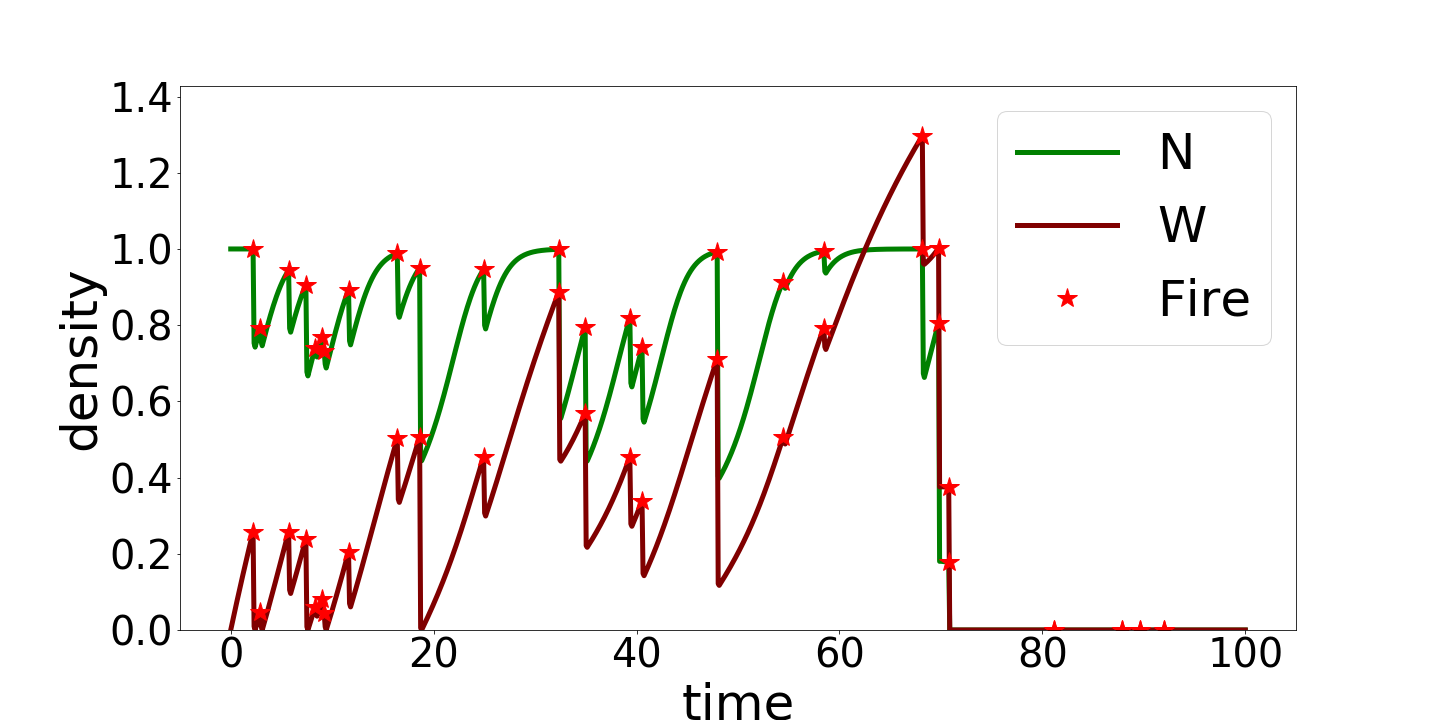
\includegraphics[width=10.cm]{time_series_1.png}}
\only<2>{
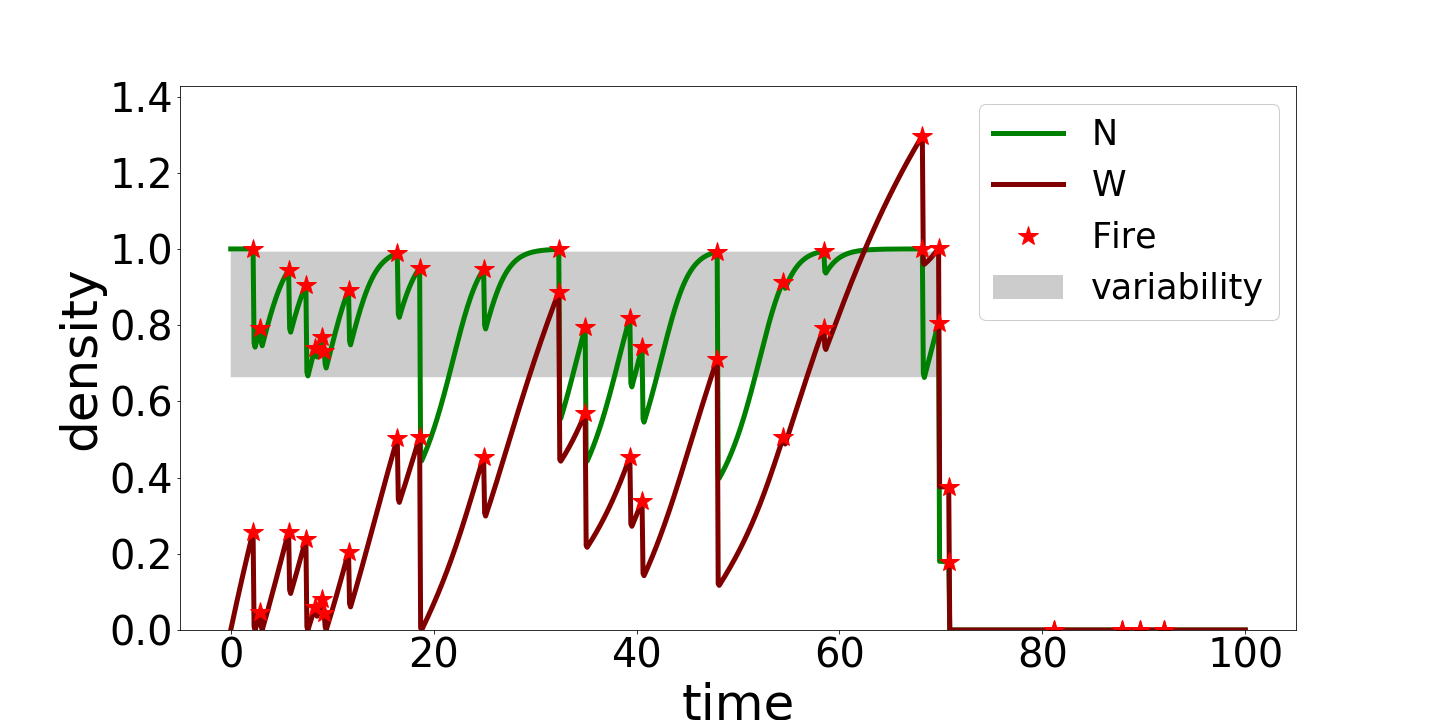
\includegraphics[width=10.cm]{time_series_sd_1.png}}
\only<3>{
%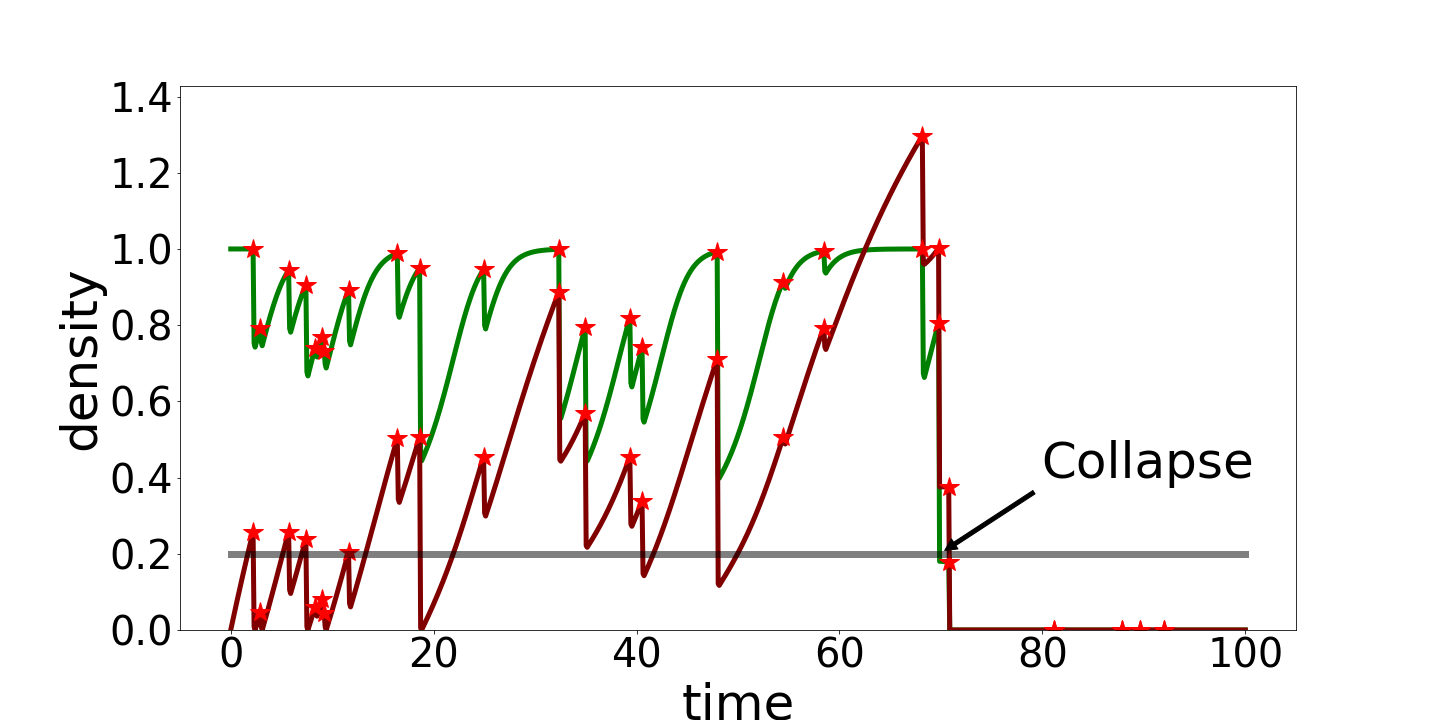
\includegraphics[width=10.cm]{time_series_cp_1.png}
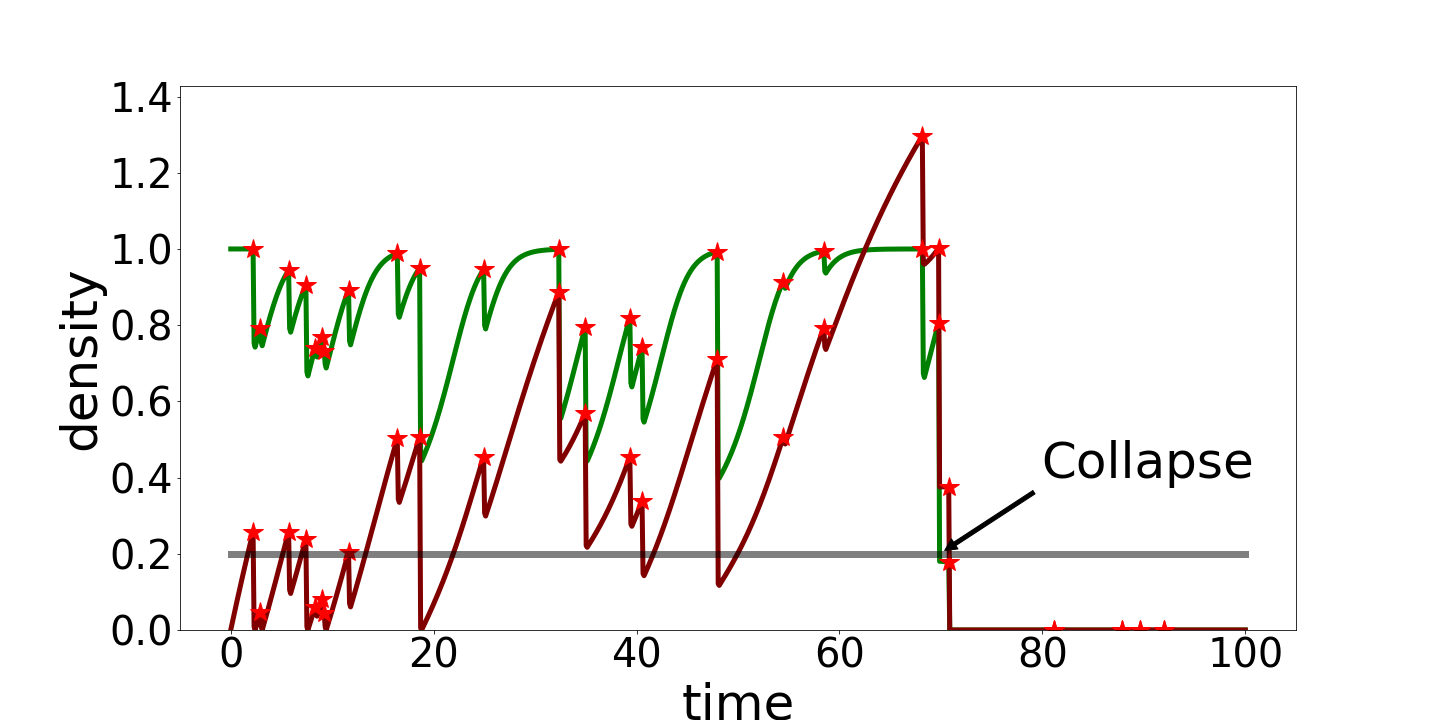
\includegraphics[width=10.cm]{time_series_cp_1.png}
}

\only<2>{
Measure variability before a collapse to avoid biases.
}
\only<3>{
Need several simulation to compute the probability to collapse.
}

\end{frame}


\section{Results}

%\subsection{frequency effects}

\begin{frame}
\frametitle{Frequency effects}
%\todo{loop : variability VS collapse probability}
\only<1>{
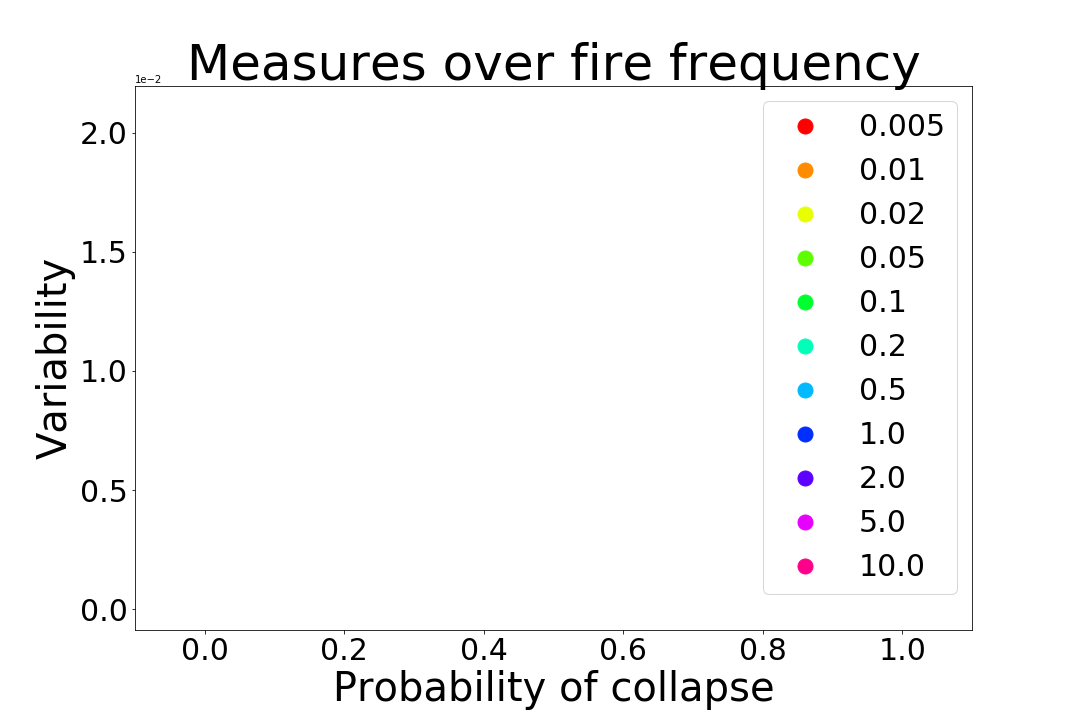
\includegraphics[width=9.cm]{loop_empty.png}
}
\only<2>{
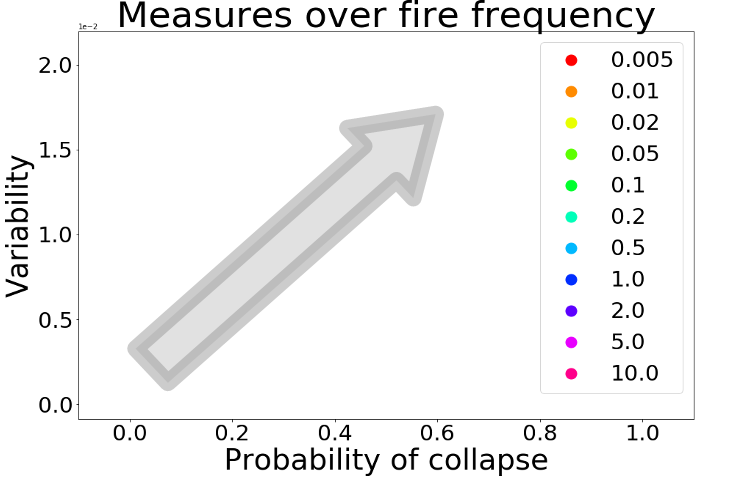
\includegraphics[width=9.cm]{loop_intuitive.png}
}
\only<3>{
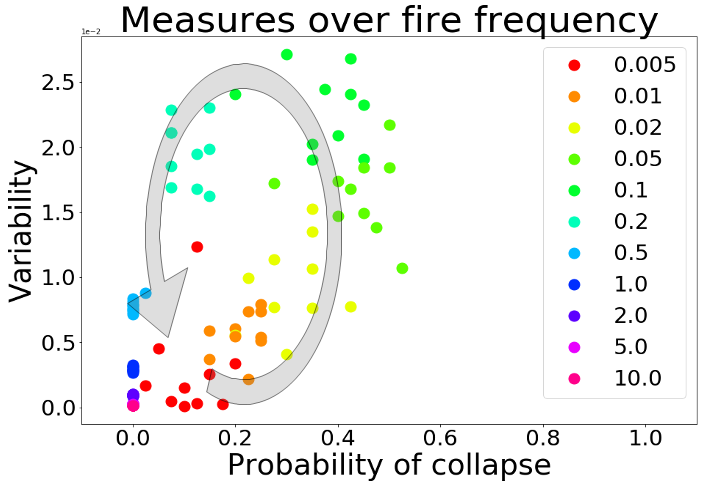
\includegraphics[width=9.cm]{loop_arrow.png}
}
\end{frame}


\begin{frame}
\frametitle{Study of the peaks}
\only<1>{
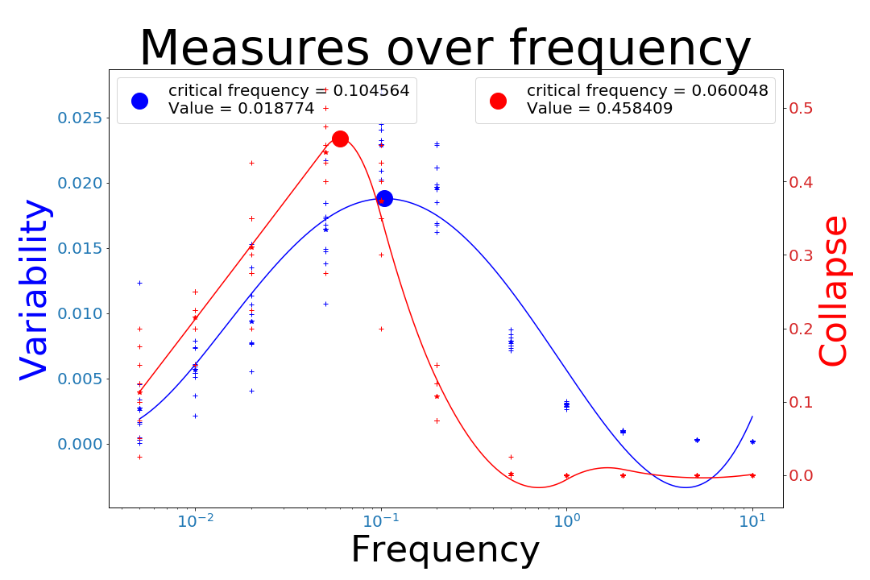
\includegraphics[width=10.cm]{peak.png}
}
\only<2>{
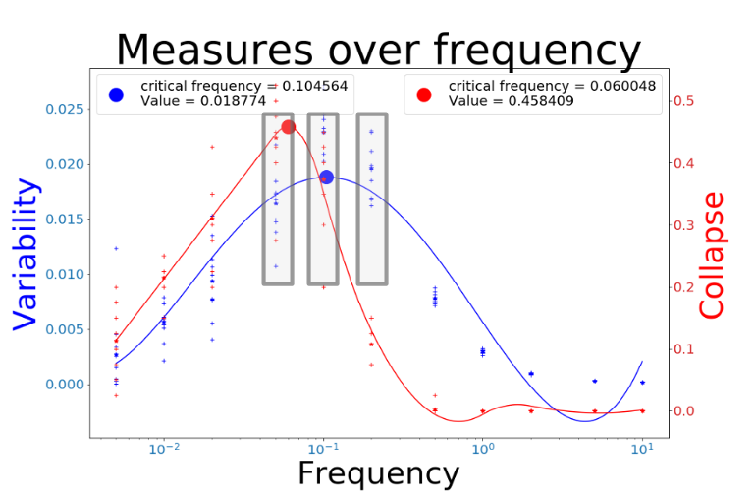
\includegraphics[width=10.cm]{peak_zone.png}
}
\end{frame}


\begin{frame}
\frametitle{Another approach}
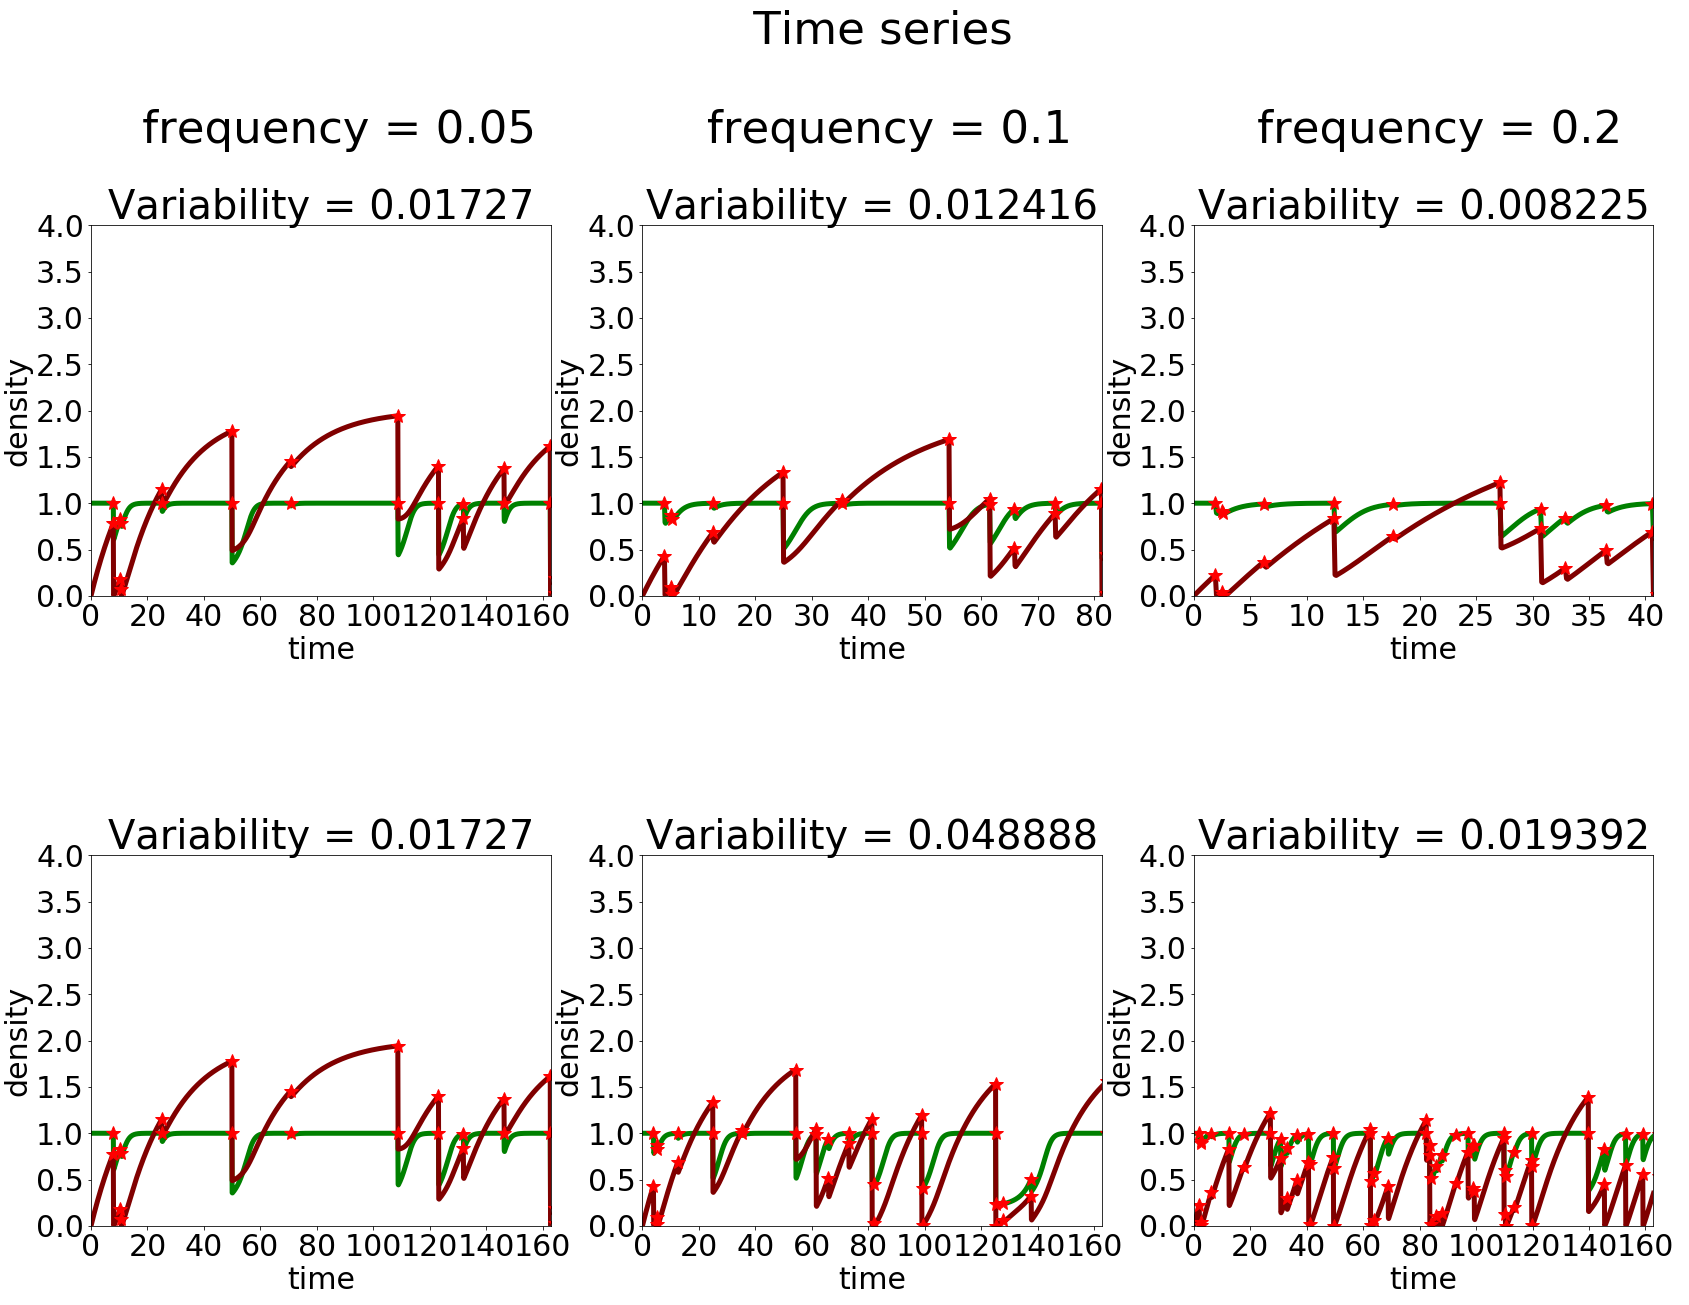
\includegraphics[width=8.5cm]{same_time_series_3.png}
\end{frame}


\begin{frame}
%\frametitle{}
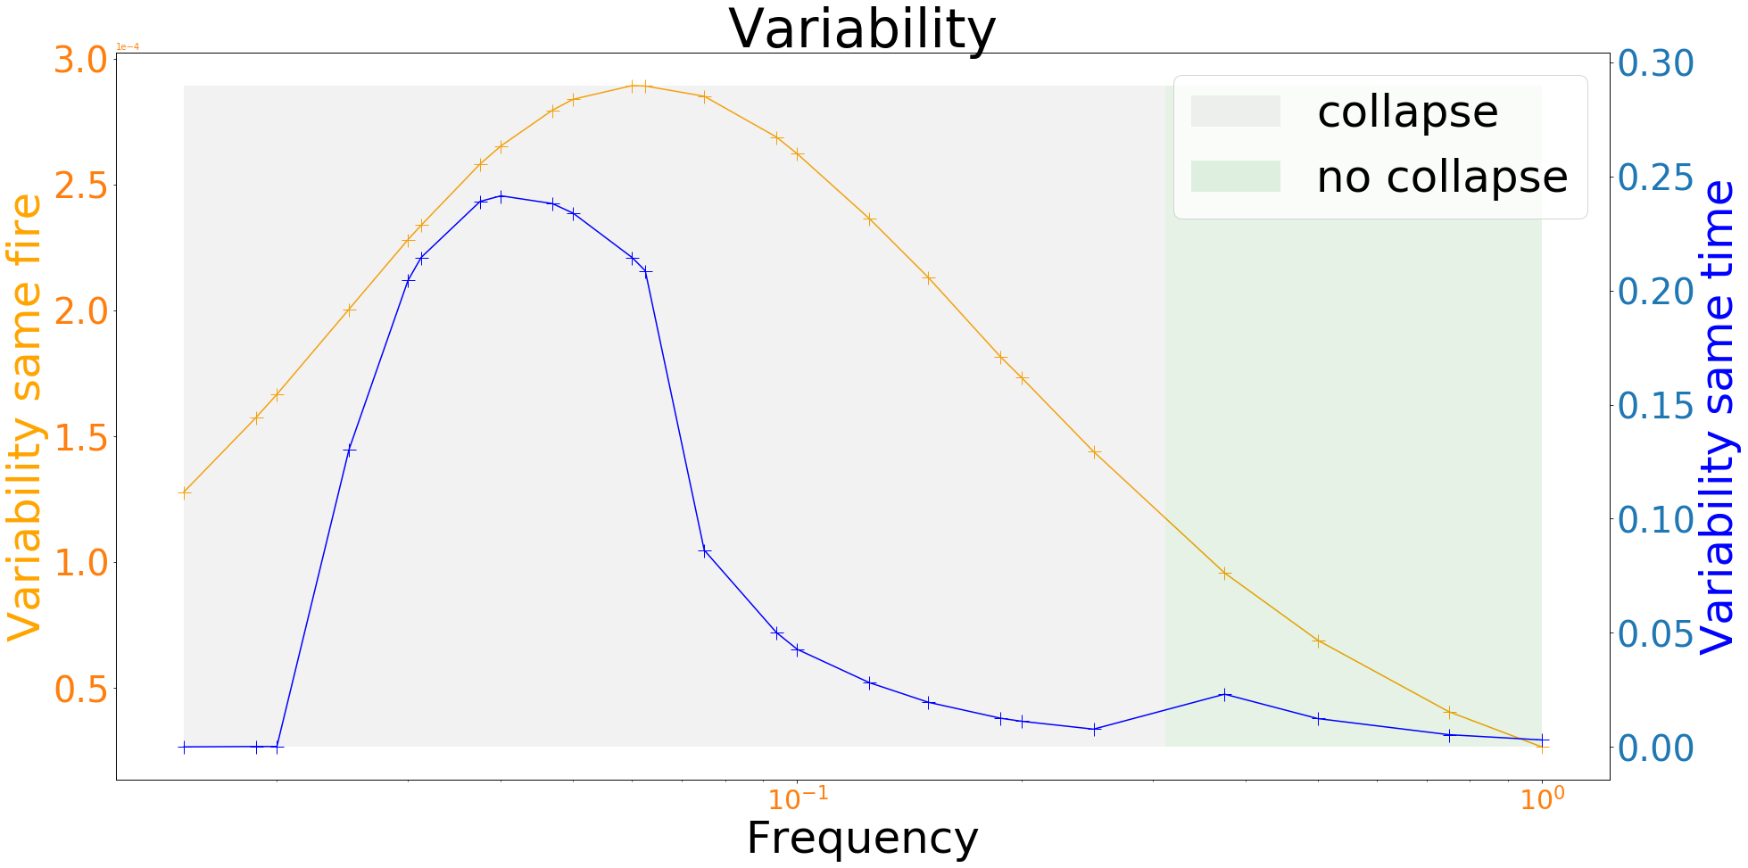
\includegraphics[width=10.cm]{var_same/5.png}
\end{frame}


\section{Conclusion}

%\subsection{Synthesis}
%\begin{frame}
%\frametitle{Synthesis}
%useful ?
%\end{frame}


\subsection{Further}
\begin{frame}
\frametitle{Further}
%\todo{list of what I am going to do after}
\begin{itemize}
    \item Explore exhaustively the various scenarios
    %\item How the shape of the loop could change ? %\todo{reformulate}
\end{itemize}
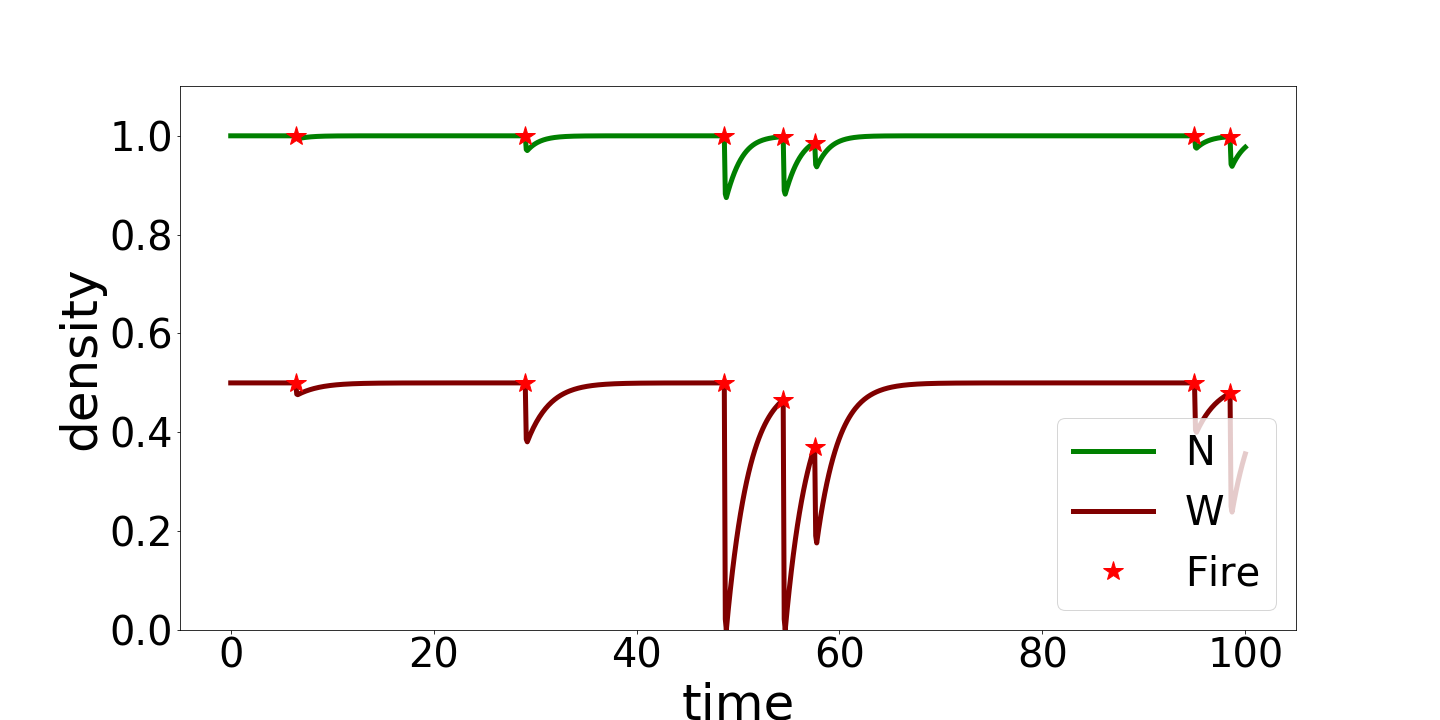
\includegraphics[width=4.cm]{1.png}
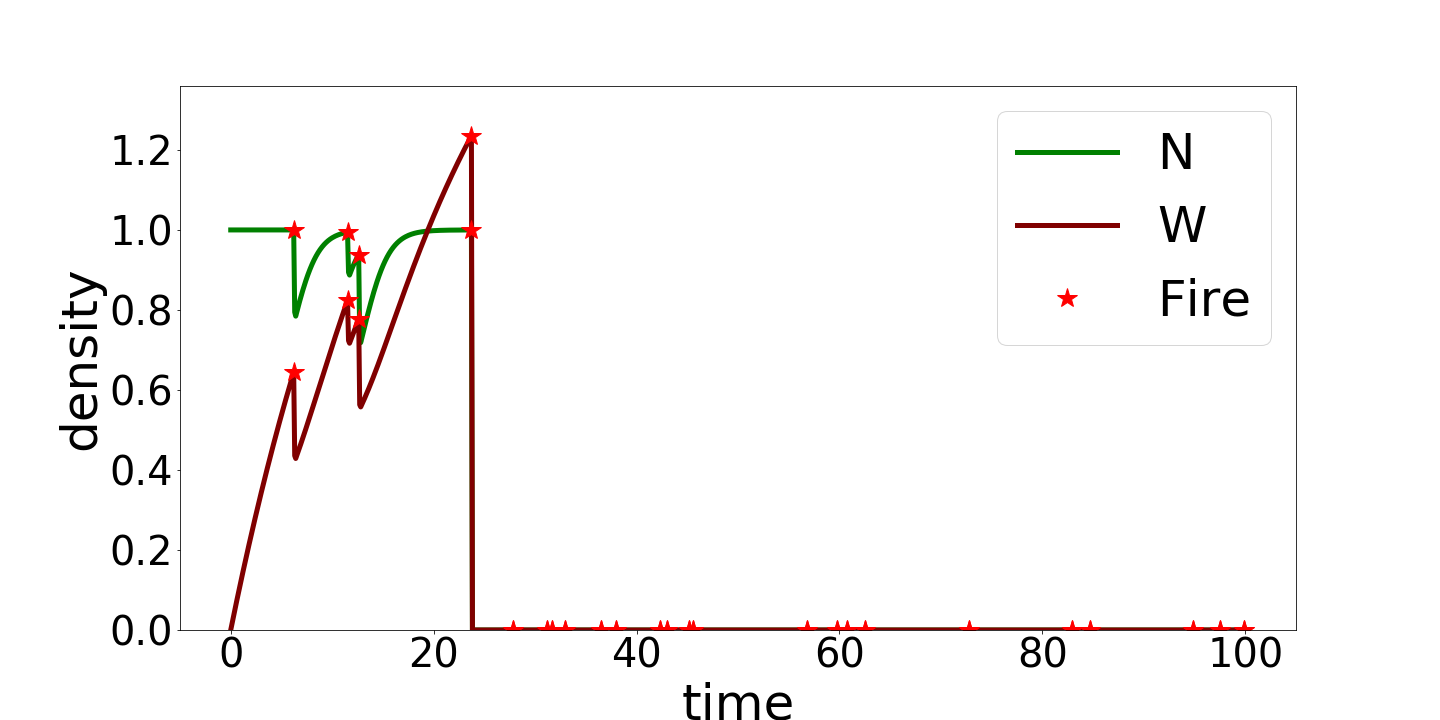
\includegraphics[width=4.cm]{2.png} \\
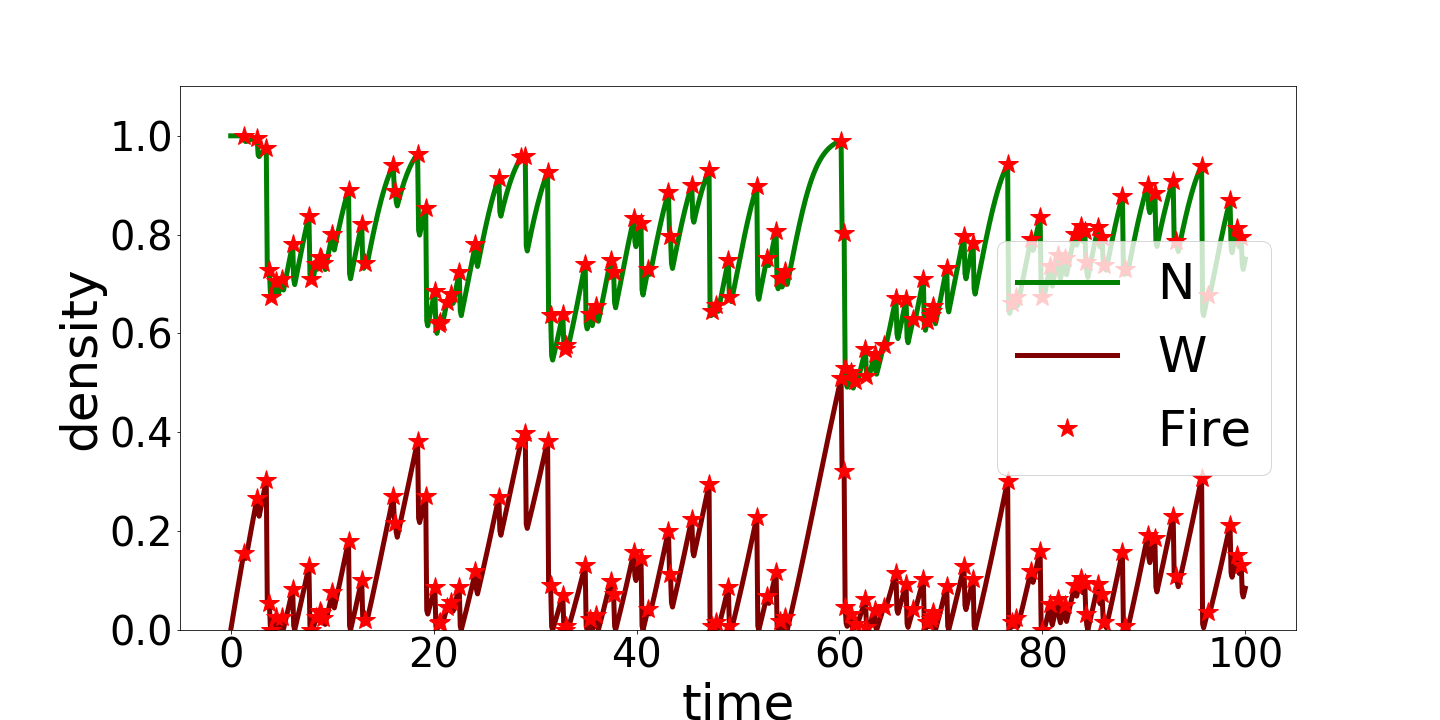
\includegraphics[width=4.cm]{3.png}
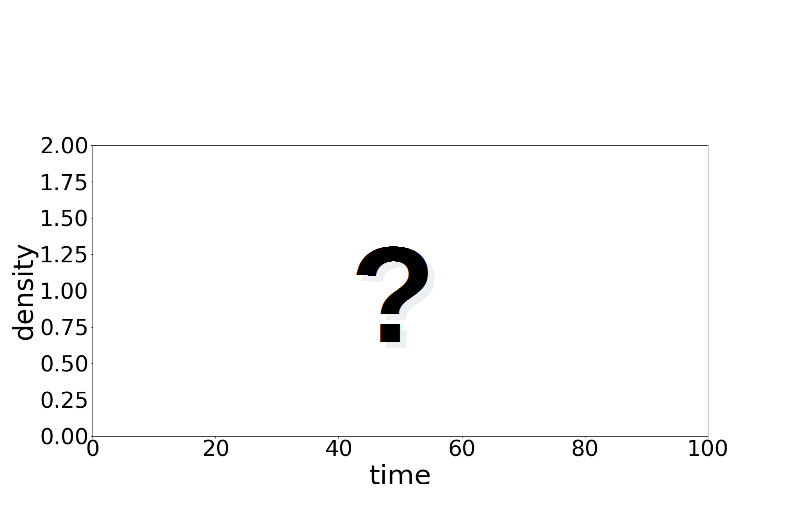
\includegraphics[width=4.cm]{4_point.png}

\begin{itemize}
    \item Why the shape of the loop could change ? %\todo{reformulate}
\end{itemize}

\end{frame}





\begin{frame}

\begin{center}
Thank you for your attention.
\\
[0.4cm]
\textcolor{red}{\rule{\linewidth}{0.5mm}} \\ 
[0.4cm]
\\
Questions ?
\end{center}

\end{frame}



\end{document}
